\chapter{Impact on force design and deterrence-by-denial} 

\begin{center}
	\begin{minipage}{0.6\textwidth}
		\centering\itshape
		The defensive is a stronger form of war than the offensive
		
		\vspace{0.5em}
		--- \textcite[ch.~V]{clausewitz_2006_on_war_project_gutenberg}
	\end{minipage}
\end{center}




The tactical changes identified in the previous chapters carry direct implications for organisational adaptation, force design and small state military utility. This chapter argues that low-cost UxS alter the relative combat power calculation in favour of a resource-constrained defender. They do so by lowering the cost of reconnaissance, precision strike and sustainment. The \textit{strategic} consequence is that an attacker must plan for a defender able to impose disproportionate cost, delay and uncertainty without matching the attacker platform-for-platform. UxS change the material conditions from which forms of deterrence may be generated. They increase the defensive value of dispersed mission command empowered light infantry. Deterrence-by-denial is treated here as an effect of altered RCP and cost imposition, rather than a theory of deterrence. This matters for Ireland because conventional mass is politically and fiscally constrained. A small state which cannot replicate the power and scale of larger militaries may still complicate an adversary's planning calculus by making lodgement, movement and sustainment costly. The question is therefore not whether UxS replace existing forces, but whether they allow small states to extract a greater defensive cost-benefit.

Unusually, Ireland has no national security strategy\index{National Security Strategy!Ireland} --- or policy per \textcite{GRAY_2018}. The Defence Policy Review therefore functions as the state's de facto defence policy\index{Defence Policy}\index{Policy!Defence}, assigning the Defence Forces the role of ``military defence of the state''  \parencite[sec. 3.2]{DPR_2024}. Without a unifying political policy and supporting defence and military strategies, the concept of ``military defence of the state'' remains notional. In that gap, the Defence Forces' Strategic Military Planning Directive provides military planning guidance, but it cannot substitute for the absent political policy framework \parencite{SMPD_2025}.


The absence of a clearly perceived external threat has reinforced an assumption that territorial defence is politically improbable, allowing force design decisions to prioritise continuity over adaptation and without articulating a \textit{theory of victory}. Yet recent developments among Western states --- most notably the United States' assertions regarding Greenland \parencite[h.~972]{us_congress_2025_congressional_record_119_1} and Denmark's response \parencite{statsministeriet_2026_faellesudtalelse_groenland} --- demonstrate that scenarios once considered implausible can rapidly acquire strategic salience. The perception of threat is an unreliable indicator for future conflict. Failure to internalise the implications of UxS risks entrenching a force posture optimised for conditions which no longer exist. UxS offer an opportunity to optimise the expenditure of toil, blood and treasure for national deterrence. Rather than consciously treating UxS as niche capabilities, the Irish Defence Forces have, through institutional inertia and strategic-cultural lag, largely failed to engage with them. It results in a de facto position of exclusion by omission despite broader efforts to restore legacy capability.

Set against the Army Force Design Office's conception of a future force \parencite{Army_force_Design,DPR_2024}, these considerations raise two interrelated questions: whether Ireland's political system will sustain significant investment in defence; and whether drone warfare alters the defensive value proposition of such equipment. The Irish Government accepted the \gls{codf} \gls{loa} 2 transformation, but funded half of the \euro3.4 billion requested \emph{for 2025--2030} \parencite{WALL_2025a}. Reports indicated that Ireland may procure armoured vehicles for circa \euro600 million \parencite{Cabirol,NOC_2026}. Estonia’s cancellation of a \euro500 million armoured vehicle programme in favour of enhanced drone defence and CUAS \parencite{ERRNews}, reflects states heeding \posscite{laboaratory} characterisation of the war; recognising that Cold War conceptions are no longer even `the last war'. As Chapter~1 argued, parity on war's outbreak requires acknowledging drones as structural modifiers of warfare --- reshaping platform utility, tactics and force design.


Technological acquisition does not in itself produce transformation. \textcite{KREPINEVICH_1994} argued that adaptation, not invention alone, determines whether innovation becomes decisive --- inter-war Britain possessed the tank concept but lacked the organisational structures to exploit it. \textcite{BETTS_1996} critiques militaries practising ``conservative progressivism'' --- embracing new systems while preserving established hierarchies and habits. \textcite[7]{rosen_1991} adds that genuine innovation requires new concepts, not merely new equipment. \textcite[11]{Davis_2014}\footnote{Writing primarily about MALE systems, though the underlying logic applies.} extends this logic to UxS, arguing that they are not transformative in isolation and require doctrinal and tactical agility to retain relative advantage. The Russo--Ukrainian War reflects this logic: UxS generated relative advantage where forces reorganised around them, creating drone units, faster kill-chains and operator-to-manufacturer adaptation loops. Revising authority structures, accelerating kill-chains and actualising mission command are more difficult than procurement \parencite{COHEN_1996,KREPINEVICH_1994}. Even where technological advantages appear evident, outcomes are determined by culture, bureaucracy, doctrine and the ability to integrate new systems into existing structures \parencite{OWENS_2002,STIMSON_2015}. Acquiring UxS does not automatically maximise RCP since the military system must evolve to realise it. Without organisational adjustment, technological integration risks generating cost without increased battlefield effectiveness \parencite{SCHAUS_2018}. As \textcite{KREPINEVICH_1994} implied, invention without reorganisation is a dead end.





Low-cost UxS create disproportionate combat power through cost imposition, fundamentally altering the deterrence calculus for resource-constrained states. Ukraine’s early resort to improvised uncrewed systems reflected necessity rather than novelty --- a logic relevant to small states with constrained conventional capability \parencite[8]{kunertova_2024_2024_08} and \parencite[10]{MOLLOY_2024}. Such systems offer asymmetric returns on investment \parencite{stu_lyle_participant_11}; for a small state such as Ireland, this supports a more credible deterrent posture under conditions of defensive resource scarcity. \textcite[10]{MOLLOY_2024} notes the emergence of coordinated drone operations, combining systems with different capabilities during a single mission. This enables multi-functional battlefield effects.

\textcite{DAVIS_e_2025} and \textcite[8]{kunertova_2024_2024_08} contend that cheap drones challenge traditional principles of force concentration and cost-benefit --- creating a ``mass effect'' of their own. \textcite{Neuberger_FP_2026} considers UAS' cost-benefit compared with tanks, GBAD and attack helicopters. Ireland's most recently procured batch of Block F Javelin ATGMs --- with a four-kilometre range --- cost circa \euro$243{,}200$. The reported $50$--$70$ kilometre FPV-OWAD\index{First Person View One-Way Attack Drone!Cost-benefit analysis versus ATGMs} range and cost warrant a comparative cost-benefit analysis. Consider the following FPV-OWAD --- treated as \emph{consumable ammunition}, per \textcite{BRONK_2024,DEVERAUX_2022,GRIFFITHS_2025} and \textcite[58]{ZABRODSKYI_2022}.

% \footnote{\textcite{MISSILES} records \$$8.7$ million for $44$ ATGMS, which corresponds to circa €10.7 million inclusive of $23$ percent Irish value added tax. This aligns with the author’s correspondence with Contracts Branch Department of Defence during 2023--2025.}

\begin{table}[H]
	\centering
	\begin{tabular}{l r}
		\toprule
		\textbf{Component} & \textbf{Cost (€)} \\
		\midrule
		13'' drone & $€742$ \\
		Fibre spool & $€38.3\,\text{km}^{-1}$ \\
		1 kg explosive & $€50\,\text{kg}^{-1}$ \\
		2 x Electric detonator & $€100\,\text{det}^{-1}$ \\
		\midrule
		Total per drone & 10 km = \textbf{$€1{,}375$} \& 70 km = \textbf{$€3{,}673$}  \\
		\bottomrule
	\end{tabular}
	\caption[Estimated tethered FPV-OWAD cost]{Estimated Fibre-Optic FPV-OWAD Cost (exclusive of VAT), per \textcite{FPV_cost_spool,FPV_cost1,FPV_cost}} \label{javcost}
\end{table}

\begin{table}[H]
	\centering
	\sbox0{%
		\begin{tabular}{ccc}
			\toprule
			\textbf{Tethered OWAD Range} & \textbf{Cost Ratio} & \textbf{Range Ratio (Javelin:FPV)} \\
			\midrule
			10 km & 1:144 & 1:2.5 \\
			70 km & 1:54  & 1:17.5 \\
			\bottomrule
	\end{tabular}}%
	
	\usebox0\par\smallskip
	
	\makebox[\linewidth][c]{%
		\begin{minipage}{\wd0}
			\footnotesize
			\raggedright
			\textit{Notes:} Rounded ratios were calculated from: the Javelin Block~F unit cost \euro197,727 exclusive of VAT versus Table~\ref{javcost}'s tethered FPV-OWAD unit costs of \euro1,375 at 10\,km and \euro3,673 at 70\,kilometres; and Javelin's four-kilometre range.
		\end{minipage}%
	}
	
	\caption[Javelin versus FPV-OWAD cost comparison]{Cost and Range Ratios (exclusive of VAT): Javelin versus Fibre-Optic FPV-OWAD, per \textcite{erikdavis_participant_7} and \textcite[187]{Javelin_range}}\label{javcost1}
\end{table}

The barrier to entry for sophisticated, precision-guided munitions at scale is collapsing. US procurement indicates FPV-OWADs are being standardised as attritable munitions: the Army cites PBAS air vehicles at \$5,000 each, while a United States Marine Corps requirement targets up to 10,000 FPV-OWADs below \$4,000 per unit \parencite{us_army_2025_fpv_training_germany_2025-07_25,sam_2025_contract_fpv_2025_12_18}.

Ireland's procurement of $44$ Javelin ATGMs\footnote{The military requirement was identified as $88$ ATGMs, per a paper staffed by the author as part of the approved business case --- heightening the cost comparison.} represents a major capital commitment to a high-cost precision munition. As shown in Table~\ref{tab:atgm_fpv_comparison12}, the same budget delivers dramatically different levels of aggregate striking potential and operational redundancy when alternative OWAD solutions are considered. This heuristic comparison is not a procurement recommendation, but rather an illustration of the quantity-quality trade-offs inherent in light infantry defensive procurement. At the low-cost end, systems such as AFUA's \textit{Molniya} OWAD compress the cost-per-effect to a degree that challenges the justification for high unit-cost ATGMs on mass-effects grounds alone. Beyond cost, ATGMs' thermal signature \parencite[22]{MOLLOY_2024}, operator exposure, weight and bulk constrain employability in two key ways: they limit ammunition carriage and complicate both dismounted and mounted transport. While FPVDs may struggle to achieve K-kills, they reliably achieve M-kills, immobilising the platform and fixing it for destruction --- via CASDs or artillery.

Table \ref{javcost} elucidates that RC are significantly cheaper than tethered UAS. They are customisable on the battlefield and quite resistant to ECM. Hence they are assessed as the control-system of choice for manoeuvre warfare --- particularly for states which can achieve air supremacy and inhibit the enemy's jamming. States may prefer RC: the quickest, proven and simplest mechanism to deploy drones --- nevertheless susceptible to countermeasures.
Such cost-efficiency and flexibility are therefore contingent on the environment: \textcite[49]{MOLLOY_2024} reports that during the 2024 battle for \index{Bakhmut}\index{Jamming!Bakhmut}Bakhmut, ``they had at least $15$--$17$ EW system installations per kilometre'', often reducing the effective range to $50$ metres.

\begin{landscape}
	\section*{ATGMs versus FPV-OWADs and Loitering-OWADs}
	\begin{table}[ht]
		\centering

		
		\begin{tabular}{lrrrr|rr}
			\toprule
			\textbf{Munition} & \textbf{Unit Cost} & \textbf{Payload} & \textbf{44 ATGM budget} & \textbf{Javelin eq} & \textbf{Salvo qty} & \textbf{Salvo} \\
			& \textbf{(incl.\ VAT)} & \textbf{(kg)} & \textbf{(purchase power)} & \textbf{payload} & \textbf{(armd coy)} & \textbf{cost} \\
			\midrule
			Javelin ATGM & \euro243 k & 8 & 44 & 44 & 6 & \euro1.458M \\
			\midrule
			RC FPV-OWAD (low) & \euro836 & 1 & 12.7 k & 1,598 & 100 & \euro83 k \\
			RC FPV-OWAD (mid) & \euro1,881 & 3 & 5.6 k & 2,131 & 33 & \euro62.1 k \\
			RC FPV-OWAD (high) & \euro3,136 & 5 & 3.4 k & 2,130 & 20 & \euro62.7 k \\
			\midrule
			RC Loitering OWAD & \euro46 k & 5 & 232 & 145 & 20 & \euro920 k \\
			RC \textit{Molniya} OWAD & \euro522 & 5 & 20.4 k & 12,783 & 20 & \euro10.5 k \\
			\bottomrule
		\end{tabular}
		\vspace{4pt}
		\begin{minipage}{0.95\linewidth}
			\footnotesize
			\textit{Notes:} Two comparative criteria are applied: budget for $44$ Javelin ATGMs (€10{,}692{,}000 incl. 23 percent VAT) and the $100$ kilogram aggregate-payload equivalence.
			
			The budget-equivalent Javelin effect and salvo quantity columns are independent: the former expresses aggregate striking potential (total warhead mass) purchasable within the $44$ ATGM budget; the latter expresses the number of effectors required to defeat an armoured company per \textcite[26--28]{BRONK_2024}, irrespective of budget. 
			
			FPV-OWADs are assessed at one, three and five kilogram warhead payloads for the low-, mid- and high unit-cost variants respectively --- though all rotary-wing FPVs can carry up to $5\,\text{kg}$, reduced payload preserves manoeuvrability and effective range at lower cost points. 
			
			Salvo effect for defeat of an armoured company ($40$--$60$ percent immobilisation of $10$ vehicles) requires $100\,\text{kg}$ in shaped-charge warheads per \textcite[26--28]{BRONK_2024}. Javelin is modelled at $100$ percent kill probability, necessitating $6$ ATGMs to meet the immobilisation threshold; hit probability, terminal performance and platform survivability are otherwise not modelled for OWAD variants. 
			
			Unit costs: FPV-OWAD and Loitering OWAD per \textcite{BRONK_2024}; \textit{Molniya} per \textcite{grobovy}; Javelin per \textcite{MISSILES}. Exchange rate $1\,\text{USD} = 0.85\,\text{EUR}$ applied throughout; all euro figures include $23$ percent VAT. All OWADs have greater range than the Javelin ATGM.
		\end{minipage}
			\caption[Anti-Armour procurement heuristic]{Comparative Anti-Armour Procurement Heuristic: ATGMs versus FPV-OWADs and Loitering-OWADs}\label{tab:atgm_fpv_comparison12}
	\end{table}
\end{landscape}


Although UxS are sometimes described as a ``game changer'' \parencite{dan_participant_1}, the term is useful only if carefully bounded. Countermeasures exist: they can be jammed, spoofed, netted, shot down and mitigated by cover, camouflage and dispersion \parencite{BRONK_2025,darragh_participant_4,stu_lyle_participant_11,bob_tollast_participant_12}.  UxS do not replace conventional human forces: they cannot seize or hold terrain, and their battlefield effects depend on integration with infantry, fires, logistics and C2 \parencite{BRONK_2025,stu_lyle_participant_11,MOLLOY_2024,WATLING_2025B}. Their significance lies in the cost-benefit problem they impose: mitigation consumes resources, drones place planning \textit{constraints} and \textit{restrictions} on tactical action and they can narrow the RCP gap between the resource-constrained defender and a conventionally superior attacker. UxS are game-changing because the barrier to entry for precision strike, rapid kill-chains and persistent ISR has collapsed. Like the machine gun, drones are best understood as an evolutionary system, ultimately integrated and normalised at progressively lower tactical echelons \parencite{stu_lyle_participant_11,oliviero_halton_2026_03_11_menace_misunderstanding,john_2025_1_2}. Normalisation indicates that militaries have internalised the increased penalty of exposure and adapted structures, procurement, tactics and doctrine accordingly. UxS are therefore best understood as a \textit{critical requirement} within a force --- able to sense, strike, protect, command and sustain.

%To date, while tactically valuable and constituting devastating lethality to light infantry, drones have yet to generate decisive strategic effects in their own right. Hence, while they are likely a \textit{critical requirement} --- particularly in the Russo--Ukrainian War --- drone units are unlikely to constitute an operational centre of gravity\index{COG!See Centre of Gravity}\index{Centre of Gravity}\index{Critical Requirement}.

The effectiveness of UAS is highly variable and dependent on context, countermeasures and target type. Reported probabilities of FPVDs reaching their target vary widely: from $70$--$75$ percent in permissive conditions \parencite{dan_participant_1} and \parencite[18:15--18:50]{Bespalov_2026}, to $20$--$40$ percent or lower in contested environments \parencite[10]{WATLING_2025B} and \parencite[27]{BRONK_2024}. Survivability rates for ISR and strike drones vary similarly, reflecting differences in EW conditions, CUAS and operator proficiency \parencite{BRONK_2024,ZABRODSKYI_2022}. Tethered systems mitigate jamming but introduce new vulnerabilities, including physical severance and problems spooling, reportedly reaching failure rates as high as $50$ percent \parencite[23:50--24:05]{Ingvald_1}. For light infantry, the most consequential probability is survivability: once detected, survival rates may fall as low as $10$ percent without effective CUAS \parencite[13:17--17:50]{zandar_2025}. \textcite[2:55--4:19]{Gifford_m_2025325} observed ``that drone will hit you; if it spots you and has a good pilot, you will die''. Against armoured targets, multiple FPVDs are often required to achieve a kill, with reports suggesting that up to $20$ systems may be needed to defeat a main battle tank \parencite{BRONK_2024,stu_lyle_participant_11,watling_2025_10} --- though mobility kills are often sufficient.
The apparent low unit cost of drones can be misleading. As \textcite[25]{MOLLOY_2024} notes, achieving a desired effect often requires multiple drones, while batteries, logistics and supply constraints impose additional costs. UAS effectiveness is therefore not a function of individual system performance, but of scale, integration and the ability to absorb attrition. While FPV-OWADs have attracted disproportionate popular attention, it is dropper drones which most directly serve light infantry needs. Their reusability, payload versatility and multi-role capacity --- spanning section- and platoon-level CAS, forward logistics and route interdiction --- make them the more consequential acquisition priority for resource-constrained light forces.

\textcite{tollast_2025_11} cautions against treating cheap drone-mass as an easily replicable solution. Ukraine's model depends heavily on\index{China!Supply chain dominance} Chinese components and supply chains which many states could not readily reproduce in wartime. This limitation is reflected in recent US efforts to decouple their supply chains from China \parencite{us_house_2025_ccp_legislation}. Taiwan’s\index{Taiwan!Drone industry capacity} drone industry now produces over 120,000 units annually \parencite{economist_taiwan}, indicating that Western-aligned manufacturing capacity is emerging despite supply chain constraints.

\textcite{BRONK_2024} note that UxS deliver effects at a cost and scale unmatched by alternative capabilities --- illustrated by Table \ref{tab:atgm_fpv_comparison12}. For Ireland, the relevant comparison is not with Europe’s front-line states, which operationalise military deterrence\index{Deterrence-by-Denial} through heavily funded conventional forces and societal mobilisation. Ireland is unlikely to replicate that model \parencite[135--148]{CODF_2022}. The question is therefore whether lower-cost mechanisms --- including dispersed drone mass enabled by mission command --- can improve RCP by making lodgement, movement and sustainment more costly for an attacker. \textcite{erikdavis_participant_7} captures the point directly: ``deterrence by denial just got a lot cheaper for a lot of countries, because you can just wreak so much havoc on any kind of a mass formation''. 

For island states, potential adversaries are logistically disadvantaged. Ground intervention requires maritime or airborne entry --- which can be observed (and targeted) by UxS. \textcite{erikdavis_participant_7} considers that the requirement to establish a lodgement for ground operations constitutes a critical vulnerability for conventional forces, which can be exploited by ``non-standard forces''.  This logic is reinforced by \textcite[22]{hvizda_2025}, who note that democratised ISR and precision strike ``could complicate offensive operations in a manner resembling the current stalemate in Ukraine''. Reconnaissance can detect force-massing, degrade\index{Camouflage and Concealment} camouflage and concealment and frustrate manoeuvre. When combined with medium- or high-altitude long-endurance UAS and\index{OSINT} OSINT, this allows mobile defences to mass effects through\index{Economy of Force} economy of force and superior\index{Situational Awareness} situational awareness.

Given \'{O}glaigh na h\'{E}ireann's roots as \emph{flying columns} --- per \textcite{tombarry,Omalley_1,Omalley_2} --- Ireland’s weakness in conventional territorial defence may be partly offset by an irregular inheritance. Dispersed forces, local knowledge, concealment and mobility become more relevant when integrated with cheap precision strike. It is an opportunity to deliver credible and cost-effective denial through UAS air interdiction.










Iran's\index{Iran} March 2026 \textit{Operation Epic Fury}\index{Operation Epic Fury} retaliation exemplified a similar logic. Large numbers of comparatively inexpensive drones saturated regional air defences and forced the conservation of high-cost interceptors \parencite[4--5]{hinote_ryan_2024}, while preserving ballistic missiles for higher-value targets \parencite{bondar_2026_03_10_iran_drone_campaign_gulf}. Iran sustained a steady rhythm of drone attacks across multiple theatres, demonstrating how low-cost aerial systems can impose continuous economic, operational and psychological strain on a defender. UxS impose a cumulative cost by forcing a superior adversary to protect exposed movement and sustainment nodes over time. For a defender capable of trading space for time, attritable UGS and OWADs are crucial\index{Critical Capability!One Way Attack Drones for Attrition}. 
\textcite[138--139]{Watling_book} notes that even small salvos of loitering munitions can saturate point-defences. Predictable employment risks optimisation by the attacker, but iterative and irregular OWAD salvos can impose sustained pressure, force defensive resource allocation and generate cumulative attrition. This matters for Ireland because UxS do not need to be independently decisive to affect RCP. Repeated attacks on movement, sustainment and force protection can create material loss while also increasing political cost for casualty-averse democracies \parencite{luttwak_1996_post_heroic}. In operations planning terms, UxS exploit a political vulnerability through attrition: the attacker’s need to protect, sustain and justify the force becomes part of the defensive cost-imposition mechanism.



For small states unable to match an adversary conventionally, political bias toward short wars may create an exploitable vulnerability.\index{Short War Bias} \textcite{RAND_short_War} argue that repeated underestimation of war's duration reflects a structural bias toward rapid, low-cost victory in great-power decision-making --- the very expectation a defender can target. UxS-enabled fires and organised irregular resistance can signal that intervention will become protracted, observable and materially costly.\index{Guerrilla Resistance} The effect is not to guarantee defeat of a superior attacker. It is to undermine the assumption that victory will be quick, cheap or politically containable. Deterrence\index{Deterrence-by-Denial} therefore depends on capability, credibility and communication: Ireland must possess usable means to impose cost, field them credibly, and signal that an adversary's movement would be exposed, delayed and punished.

The cost-imposition mechanism operates through the credible communication that victory --- if achievable --- will be neither quick nor cheap. That message becomes credible when adversary staff assess RCP and advise that the operation may generate politically unacceptable costs. \posscite[22]{Aus_defences_strat_2024} strategy of denial is instructive because it frames denial as a signal of credible military capacity, not simply a battlefield outcome:\index{Denial!Strategy of}\index{Australian Government!Strategy of denial} ``designed to deter\index{Deterrence-by-Denial!Australian strategy of} a potential adversary from taking actions [and] signalling a credible ability [to] deter attempts to coerce Australia through force''. For Ireland, the implication is narrower but relevant: UxS-enabled cost imposition can support denial by raising the expected costs.


\textcite{MURRAY_2008} argued that Taiwan\index{Taiwan} should reject symmetric competition in favour of denial and cost-imposition through a distributed \textit{porcupine strategy}\index{Porcupine Strategy!Taiwan}. \textcite{paparo} later articulated a comparable operational approach, describing the saturation of the \index{Taiwan Strait}Taiwan Strait with UxS to deny a rapid, low-cost victory. More recently, \textcite{CSIS_Taiwan_ROC,pettyjohn} shift the question from whether Taiwan can win conventionally to whether an adversary can absorb the chaos, casualties and uncertainty imposed by such a defence. The transferable lesson is that denial works by making rapid victory uncertain, not by matching the adversary symmetrically.

For Ireland, the equivalent mechanism is not a porcupine strategy, but dispersed light infantry enabled by mission command and integrated UxS. Such a force would be difficult to track en masse, particularly in increasingly urbanised terrain \parencite[ii]{future_cities}. It could deliver the protraction and attrition required to undermine great-power short-war assumptions. For a small state lacking conventional depth, this force represents both the mechanism of cost-imposition and the credible signal that territorial coercion would be neither quick nor cheap. \textcite{Williams_2022_3_31} highlights early United States Marine Corps observations that drones, loitering munitions and light mobility platforms enable light infantry to impose disproportionate costs on heavier mechanised forces without maintaining comparable armoured capabilities. Subsequent combat has borne this out.

This does not make UxS a substitute for infantry. \textcite[6:05--12:55]{Leach_curtain} argues that ``we must stop minimising the importance of [well trained] infantry'' and other conventional weapons. Drone teams require defence and without infantry, the adversary would exploit this vulnerability \parencite[7:00--7:30]{Leach_curtain}. The introduction of guided ATGMs, for example, was once considered to signal the end of the main battle tank. In practice, however, massed artillery and manoeuvre displaced firing positions and degraded their battlefield effect \parencite{stu_lyle_participant_11}. UAS teams are subject to similar pressures: their effectiveness can be reduced through suppression, the disruption of their logistics or control nodes and manoeuvre --- as evidenced by contemporary Russian practice \parencite[3]{watling_2025_10}. 

Given that most contemporary UxS remain dependent on radio or satellite connectivity, lost communications risks converting a drone-centric defence into a liability, exposing insufficient infantry depth  \parencite{Axe_sound_of_silence_2026} --- exemplified by Russia’s 2026 communications collapse \parencite{Axe_starlink_2026}\index{Telegram!Removal from AFRF communications}\index{Starlink!Removal from AFRF communications}\index{Discord!Removal from AFRF communications}\index{Armed Forces of the Russian Federation!Starlink shut-off}\index{Armed Forces of the Russian Federation!Messaging applications prohibition}. Autonomous terminal guidance has been anecdotally reported in some systems. Fully autonomous cooperative swarms, however, have not yet been observed in operational use. Their emergence, discussed by \textcite{civdiv_12}, would significantly alter current assessments of UAS dependence on communications links. 

As \textcite[19:00--20:50]{Ingvald} observe ``you cannot win a war with just drones'', a conclusion echoed by \textcite[25]{MOLLOY_2024} and \parencite{BRONK_2025}. UxS remain enablers rather than substitutes for combined arms forces \parencite{BRONK_2022a,BRONK_2025,CORNISH_2024,Radec,WATLING_2023A,WATLING_2023B,WATLING_2024A,WATLING_2025B}. For a small state designing deterrence\index{Deterrence-by-Denial!Centred around armed UxS} around armed UAS, the implication is clear: resilience, not acquisition, is decisive.  Redundancy is essential: resilient communications, decentralised stockpiles and mission-command empowered infantry. Without these, drone-enabled deterrence becomes a vulnerability.

The communications problem may be less one of capability than of signature: proliferating cheap, low-power, disposable technologies that hide within civilian electromagnetic noise may prove more survivable than exquisite systems that advertise their presence to an AI-enabled adversary \parencite[9,~18]{Birchfield_2026,USMC_MOC_2016}.

Concurrently, \textcite{dan_participant_1,Leach_curtain} note\footnote{Confer \textcite{civdiv_2024_10_05} for a battlefield depiction.}, drone teams must have a high level of infantry skills to begin with --- for infiltration and defence against adversary raids. In functional terms, this aligns them closely with light infantry roles; hence, drone teams \textit{are a form of infantry} with an ``outsize tactical value'' \parencite[26]{hvizda_2025}.


Effective employment of UAS depends on organisational concentration at higher echelons combined with controlled decentralisation at lower levels. The battlefield effectiveness of Magyar's Birds\index{Magyar's Birds} and Rubicon Centre\index{Rubicon Centre} indicates that armed drones are most effective when concentrated in dedicated units capable of mass and rapid repositioning. These observations indicate a requirement for brigade-level UAS formations. Ukrainian practice reflects this trend: the national police's Joint Assault Brigade \textit{Lyut} fields the \textit{Kruk} battalion to disrupt enemy logistics \parencite{NPU_Lyut_Kruk_2026}, while the Fury Brigade integrates armed and unarmed UAS and UGS \parencite{Militarnyi_Kruk_2026}, demonstrating the institutionalisation of UxS at scale.

Force design is therefore a question of structure and institutional permission. The challenge is not whether drones require regulation, but whether they are regulated in a way that preserves scale, attritability and adaptation. \textcite{goc_participant_3} contends that oversight, training and accountability remain necessary. However, applying the administrative logic of conventional aviation to small battlefield drones --- many of which are best considered consumables --- risks suppressing the attributes on which their combat value depends \parencite[57--58]{ZABRODSKYI_2022} and \parencite[51:30--54:15]{WATLING_2023_book_launch}. In peacetime, this creates a particular danger: institutional inertia can prevent adaptation until combat imposes it at greater cost.

At lower echelons, the offensive corollary is a mixed organic capability. FPV-OWADs offer range but are single-use, whereas CASDs are reusable but lack equivalent stand-off. A complementary mix is therefore indicated, with stabilised CASDs possessing sufficient utility to warrant decentralised use, such that infantry develop baseline proficiency \parencite[24:00--25:00]{Leach_curtain}.

\index{Force Design!Battalion-level CUAS}This organisational logic must be replicated for countermeasures. \textcite[2]{WATLING_2024} argue for battalion-level CUAS/anti-aircraft systems and brigade-level CUAS units. The vulnerability of static positions to UAS attack --- illustrated by Iranian strikes during Operation Epic Fury\index{Operation Epic Fury} \parencite{aljazeera_2026_03_15_fpv_drone_us_base_iraq} --- reinforces that reliance on higher-echelon protection is insufficient. Effective battalion design therefore requires an integrated approach combining concentrated UAS mass, decentralised employment and organic CUAS.

Below battalion level, a tension arises between concentration and decentralisation.\index{Force Design!Company-level armed UAS} UAS are relatively fragile, logistically demanding and operator-intensive \parencite{dan_participant_1,dan_participant_6}, indicating that effective employment requires dedicated teams rather than dispersal across manoeuvre elements. This reinforces the need for protected operators and local security, further binding UAS employment to infantry. The increasing technical and cognitive demands of modern warfare also raise training thresholds, with estimates suggesting that minimum infantry training now exceeds twenty weeks \parencite{watling_2025_panel,darragh_participant_4}. 

\index{Force Design!Armed UGS in the battalion}UGS enable partial decentralisation of heavy firepower. \textcite[40:00--42:00]{lyle_23_interview} suggests that weaponised UGS could deliver effects comparable to organic armoured support at company level, potentially redistributing capabilities previously held at brigade. 
However, the logistical and operational characteristics of UGS differ sharply from expendable UAS. Greater size and weight, drivetrain maintenance, battery dependency, armour integration, exposure to direct and indirect fires and their non-consumable nature render organic platoon-level inclusion impractical\index{UGS!Battalion- and company-level incorporation}. Their management more closely resembles that of vehicle fleets than expendable UAS. UGS are therefore best assessed as battalion-level assets, held within the support and headquarters companies. Limited allocation to light rifle companies for logistics is prudent. This assessment is consistent with the thematic analysis and reflects a broader requirement for organic all-terrain lift capacity within infantry companies, a role which UGS in a logistics function may partially fulfil.



These developments also challenge the traditional structure of the Support Company. The continued separation of anti-armour capability into a dedicated platoon is increasingly questionable. A reorganisation toward UxS --- including the establishment of a CASD platoon and the partial conversion of anti-armour and reconnaissance elements --- better reflects contemporary battlefield dynamics. Earlier reform proposals, such as \textcite{egerton_2021}, anticipated the integration of ISRDs but did not foresee its pervasive effect on lethality.

This logic has direct implications for the internal structure of the battalion, particularly at company and section levels. A more ambitious design inverts the traditional logic: the assault detachment is built around the FPVD --- as the machine gun once became the organising weapon of the infantry section. Given FPVD's demonstrated value for reconnaissance, precision strike and protected lethality, and the acute vulnerability of pilots when flying, this reorientation is analytically justified.\index{Force Design!Building the detachment around the FPVD}

Figure~\ref{fpvdet} presents the resulting fifteen-soldier section. The first assault detachment pairs an FPVD operator with three rifles under a lance corporal, providing protection and enabling concealed operation. The second retains the machine gun, preserving organic suppression. The support detachment integrates ISRD, CUAS, assault pioneer and rifle under a fourth lance corporal. It is more demanding in training and procurement than the nine-soldier model. It is also more flexible --- and lethal.

\begin{figure}[H]
	\centering
	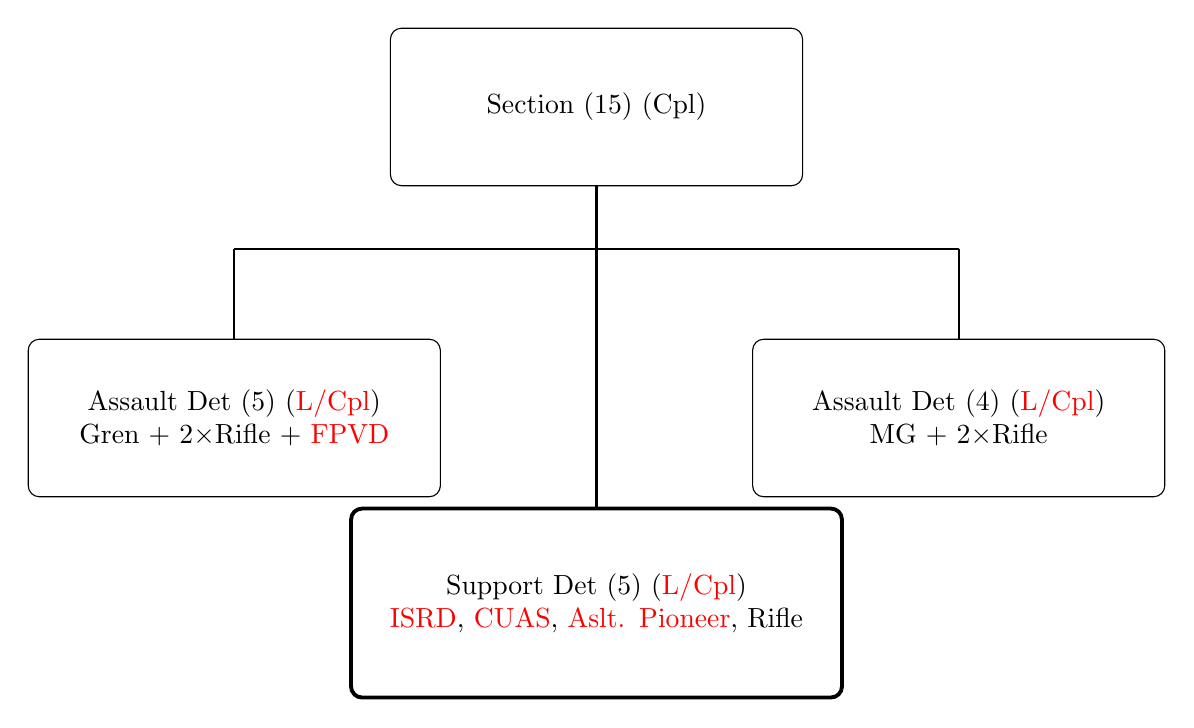
\begin{tikzpicture}[
		box/.style={
			draw,
			rounded corners,
			align=center,
			minimum width=5.2cm,
			minimum height=2cm,
			text width=5cm,
			font=\normalsize,
			fill=white
		},
		supportbox/.style={
			draw,
			rounded corners,
			line width=1.4pt,          % thicker border
			align=center,
			minimum width=6.2cm,       % wider
			minimum height=2.4cm,      % taller
			text width=6cm,
			font=\normalsize,%\bfseries, % bold text
			fill=white                 % no shading
		},
		line/.style={draw, thick}
		]
		
		% Section commander
		\node[box, minimum width=3.8cm] (sec) at (0,0) {Section (15) (Cpl)};
		
		% Assault detachments
		\node[box] (ass1) at (-4.6,-3.95) 
		{Assault Det (5) (\textcolor{red}{L/Cpl})\\Gren + 2$\times$Rifle + \textcolor{red}{FPVD}};
		
		\node[box] (ass2) at (4.6,-3.95) 
		{Assault Det (4) (\textcolor{red}{L/Cpl})\\MG + 2$\times$Rifle};
		
		% Support detachment (larger + thicker + bold)
		\node[supportbox] (sup) at (0,-6.3) 
		{Support Det (5) (\textcolor{red}{L/Cpl})\\\textcolor{red}{ISRD}, \textcolor{red}{CUAS}, \textcolor{red}{Aslt. Pioneer}, Rifle};
		
		% Structure lines
		\draw[line] (sec.south) -- (0,-1.8);
		\draw[line] (-4.6,-1.8) -- (4.6,-1.8);
		\draw[line] (-4.6,-1.8) -- (ass1.north);
		\draw[line] (4.6,-1.8) -- (ass2.north);
		\draw[line] (0,-1.8) -- (sup.north);
		
	\end{tikzpicture}
	\caption[15 soldier section structure: modern warfare]{Section structure 3: Fifteen-soldier section with organic FPVD, support detachment and separate commander}
	\label{fpvdet}
\end{figure}

%\section{Conclusion}
This chapter has argued that UxS alter the cost structure of defensive RCP in ways directly relevant to Ireland’s strategic position.\index{\index{Deterrence-by-Denial}!Cost structure} The Javelin-to-FPV cost ratio --- 1:54 to 1:144 depending on range --- shows that mass precision effect is no longer the preserve of well-funded conventional forces.\index{Cost-Benefit!Javelin versus FPV-OWAD} For a small island state whose irregular warfare heritage predates its conventional one, and whose political system has consistently declined to fund conventional mass at scale, UxS offer an alternative route to defensive utility.

The argument is not that drones replace conventional power. Rather, UxS can partially substitute for mass in selected defensive functions. They can make lodgement, movement, sustainment and consolidation more observable, targetable, delayed and costly. In doing so, they improve RCP by forcing an attacker to plan against a force able to impose cumulative cost without matching the attacker platform-for-platform.

That effect is only credible when UxS are integrated into a resilient force. Mission-command empowered light infantry remain the foundation. A drone-first posture built on fragile communications, foreign supply chains and insufficient infantry depth is therefore a vulnerability as much as a capability. Credible denial requires redundancy: resilient command, decentralised stockpiles, organic hard-kill CUAS, protected drone teams, secure supply and sustained political investment.

The central implication is therefore politico-strategic rather than technological. Ireland does not lack access to the basic technologies required to begin adapting. It lacks the strategic architecture, institutional urgency and political commitment required to convert those technologies into combat power. UxS do not solve Ireland’s defence problem, but they clarify it: a small state can no longer justify weak territorial defence on the basis that credible combat power is financially unreachable.

